%% Appendix B (Robustness). 


This appendix reports the robustness exercise summarized in \autoref{sec:results_rob} in full. We vary, one at a time, each of the four ingredients that could in principle change the rotation rather than reveal it: the measure of the Fed's stance, which determines the regime allocation; the measure of the euro area policy surprise, which determines the impulse; and the two transition parameters. \autoref{tab:robspecs} lists the resulting specifications, the share of weeks it assigns to the restrictive regime, and the correlation of its posterior
median impulse responses with the baseline.

\textcolor{blue}{comment out the code name column. remove the steepness prior row.}
\begin{table}[!htpb]
\caption{Robustness specifications.\label{tab:robspecs}}
\centering \footnotesize
\resizebox{\textwidth}{!}{% generated by Results/diagnostics/make_robustness_tables.R
% 2026-07-27 (by hand): code-name column removed; "neutral cut" renamed "neutral stance".
% Code names retained as end-of-row comments for the replication package.
\begin{tabular}{lrr}
\hline\hline
Change relative to the baseline & Restrictive & Corr. with \\
 & share & baseline IRFs \\
\hline
Baseline: $DFF-r^\ast$ stance, four-factor surprise, $\mu=0$, $\rho\sim G(4000,1000)$ & 41.0\% & 1.000 \\ % main
Stance replaced by the Krippner shadow short rate less $r^\ast$ & 41.0\% & 0.973 \\ % ssr
Surprise replaced by \cite{jarocinski2020deconstructing} median-rotation shocks & 41.0\% & 0.769 \\ % jk
Neutral stance lowered to $-0.50$ pp & 54.6\% & 0.994 \\ % zlo50
Neutral stance lowered to $-0.25$ pp & 46.6\% & 0.998 \\ % zlo25
Neutral stance raised to $+0.25$ pp & 37.7\% & 0.999 \\ % zhi25
Neutral stance raised to $+0.50$ pp & 34.8\% & 0.994 \\ % zhi50
Steepness prior centred at $7$ instead of $4$ & 41.0\% & 0.998 \\ % rho7
\hline\hline
\end{tabular}
}
\caption*{\footnotesize \textit{Notes:} Each specification alters exactly one ingredient of the baseline and leaves the remainder unchanged. The restrictive share is the fraction of weeks with posterior mean $S_t > 0.5$. The final column is the correlation between the posterior median yield responses of the specification and those of the baseline, taken across all maturities, stance percentiles and horizons. Note that the correlation is not directly comparable for \texttt{jk}, whose surprise series is a different object with a different scale.}
\end{table}

\autoref{tab:robgap} reports the state dependence itself: the difference between the response at the fifth and at the ninety-fifth percentile of the stance, and the posterior probability that this difference is positive. The sign and the maturity profile are common to every specification. The
gap is negative at one year, indistinguishable from zero, and positive
and increasing in maturity from ten years out, where the posterior probability of a positive gap is at least $0.92$ in seven of the eight specifications and $0.82$ in the eighth. Its magnitude, however, varies by a factor of more than three across specifications, and we accordingly make no claim about the size of the effect in the main text.

\begin{table}[!htpb]
\caption{The state-dependence gap across specifications.\label{tab:robgap}}
\centering \footnotesize
\resizebox{\textwidth}{!}{% generated by Results/diagnostics/make_robustness_tables.R -- do not edit by hand
\begin{tabular}{lrrrrrrrr}
\hline\hline
Maturity & Baseline & SSR $-r^\ast$ & JK shocks & $\mu=-0.50$ & $\mu=-0.25$ & $\mu=+0.25$ & $\mu=+0.50$ & $\rho$ prior $7$ \\
\hline
\multicolumn{9}{l}{\textit{1 year}} \\
 \quad median gap & -0.46 & -0.80 & -0.50 & -0.58 & -0.57 & -0.32 & -0.09 & -0.52 \\
 \quad $P(\text{gap}>0)$ & 0.26 & 0.12 & 0.27 & 0.23 & 0.23 & 0.33 & 0.44 & 0.21 \\
\multicolumn{9}{l}{\textit{3 years}} \\
 \quad median gap & -0.28 & -1.15 & -0.02 & -0.25 & -0.31 & -0.16 & 0.02 & -0.45 \\
 \quad $P(\text{gap}>0)$ & 0.36 & 0.07 & 0.49 & 0.39 & 0.34 & 0.42 & 0.52 & 0.26 \\
\multicolumn{9}{l}{\textit{5 years}} \\
 \quad median gap & 0.10 & -0.75 & 0.17 & 0.18 & 0.11 & 0.16 & 0.25 & -0.06 \\
 \quad $P(\text{gap}>0)$ & 0.55 & 0.15 & 0.64 & 0.59 & 0.56 & 0.59 & 0.64 & 0.46 \\
\multicolumn{9}{l}{\textit{10 years}} \\
 \quad median gap & 0.63 & 0.05 & 0.36 & 0.76 & 0.68 & 0.58 & 0.53 & 0.56 \\
 \quad $P(\text{gap}>0)$ & 0.85 & 0.53 & 0.77 & 0.85 & 0.85 & 0.84 & 0.82 & 0.85 \\
\multicolumn{9}{l}{\textit{15 years}} \\
 \quad median gap & 0.85 & 0.37 & 0.43 & 0.99 & 0.91 & 0.76 & 0.65 & 0.83 \\
 \quad $P(\text{gap}>0)$ & 0.93 & 0.75 & 0.80 & 0.91 & 0.92 & 0.91 & 0.87 & 0.94 \\
\multicolumn{9}{l}{\textit{30 years}} \\
 \quad median gap & 1.08 & 0.71 & 0.48 & 1.22 & 1.16 & 0.96 & 0.79 & 1.08 \\
 \quad $P(\text{gap}>0)$ & 0.97 & 0.89 & 0.81 & 0.96 & 0.97 & 0.95 & 0.90 & 0.98 \\
\hline\hline
\end{tabular}
}
\caption*{\footnotesize \textit{Notes:} The gap is the one-week-ahead response at the fifth percentile of the Fed's stance less the response at the ninety-fifth percentile, in basis points per one standard deviation euro area surprise, computed draw by draw. $P(\text{gap}>0)$ is the share of posterior draws in which the gap is positive. Because the surprise is standardized within each specification, magnitudes are comparable across all columns except \texttt{jk}, whose underlying series has a standard deviation of $3.5$ rather than $5.7$ basis points; for that column the sign and the maturity profile are informative but the level is not.}
\end{table}

\autoref{tab:robrot} states the rotation directly. Panel A records, for each maturity, the highest percentile of the Fed's stance at which the response is still significantly positive; reading down a column traces the rotation, since a response that survives at every percentile at short maturities but fails beyond the fiftieth or sixtieth at long maturities is precisely a curve that pivots rather than shifts. Panel B records the lowest percentile at which the response has become significantly
negative. The distinction matters: an unsigned test that merely asked whether the credible band excludes zero would treat a significantly negative long-end response as though the response were robustly present, when in fact it is the strongest form of the rotation. In three specifications the thirty-year response does turn significantly negative once the Fed is sufficiently restrictive.

\textcolor{blue}{remove panel B as it is everywhere the same result. just mention one sentence in the paragraph above}
\begin{table}[!htpb]
\caption{The rotation: signed significance frontier.\label{tab:robrot}}
\centering \footnotesize
\resizebox{\textwidth}{!}{% generated by Results/diagnostics/make_robustness_tables.R
% 2026-07-27 (by hand): Panel B (negative frontier) removed -- it is "--" for every
% specification at every maturity under seed 1002; the point is now made in one sentence
% in the appendix text.
\begin{tabular}{lrrrrrrrr}
\hline\hline
Maturity & Baseline & SSR $-r^\ast$ & JK shocks & $\mu=-0.50$ & $\mu=-0.25$ & $\mu=+0.25$ & $\mu=+0.50$ & $\rho$ prior $7$ \\
\hline
1 year & 100 & 100 & 100 & 100 & 100 & 100 & 100 & 100 \\
3 years & 100 & 100 & 100 & 100 & 100 & 100 & 100 & 100 \\
5 years & 100 & 100 & 100 & 100 & 100 & 100 & 100 & 100 \\
10 years & 100 & 100 & 70 & 100 & 100 & 100 & 100 & 100 \\
15 years & 100 & 100 & 60 & 100 & 100 & 100 & 100 & 100 \\
30 years & 65 & 70 & 55 & 65 & 65 & 70 & 70 & 60 \\
\hline\hline
\end{tabular}
}
\caption*{\footnotesize \textit{Notes:} Entries are percentiles of the Fed's stance distribution.
Panel~A gives the highest percentile at which the sixteenth posterior quantile of the response is
still above zero, Panel~B the lowest percentile at which the eighty-fourth quantile has fallen
below zero. ``--'' indicates that the condition is never met. A value of $100$ in Panel~A means
the response remains significantly positive across the entire stance distribution.}
\end{table}

\textcolor{blue}{cut is missleading. work with neutral stance and change everything accordingly here}
Finally, \autoref{fig:zetafrontier} isolates the dependence on the calibrated neutral stance. Lowering the neutral stance confines the accommodative state to more deeply accommodative weeks and widens the estimated gap; raising it has
the opposite effect. What the figure also shows, however, is that the credible band lies entirely above zero over the whole range considered, at both maturities: the existence of the state dependence does not turn on where the boundary is placed, only its measured size does.

\begin{figure}[!htpb]
\caption{The state-dependence gap as a function of the calibrated neutral
stance.\label{fig:zetafrontier}}
\centering
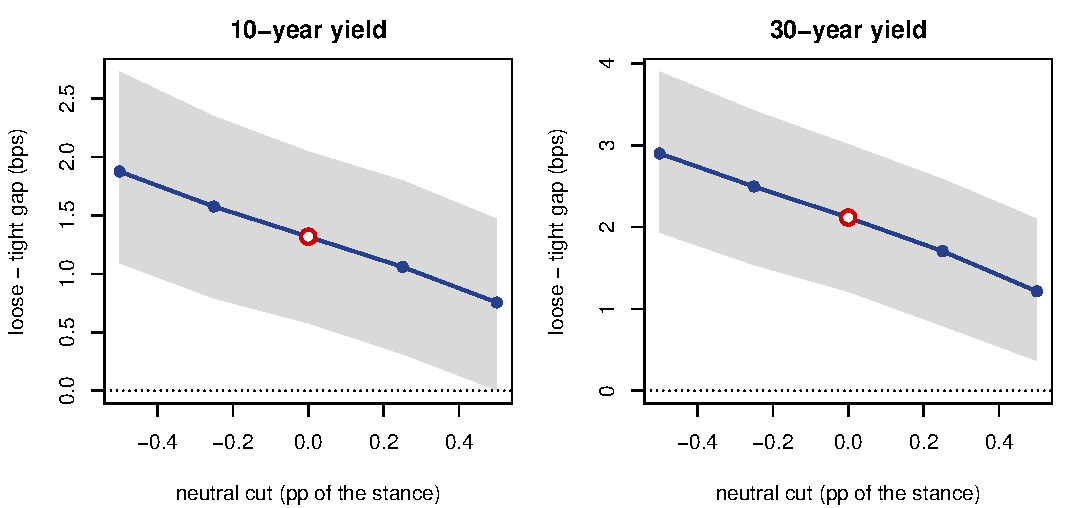
\includegraphics[width=\textwidth]{images_updated/rob/zeta_frontier.pdf}
\caption*{\footnotesize \textit{Notes:} Posterior median (solid line) and $68\%$ credible band
(shaded) of the loose-minus-tight gap in the one-week-ahead yield response, plotted against the
calibrated neutral cut $\mu$ in percentage points of the Fed's stance. The open red circle marks
the baseline calibration $\mu=0$, at which the restrictive regime comprises $41.0\%$ of weeks; the
end points $\mu=\mp0.50$ correspond to $54.6\%$ and $34.8\%$ respectively. Left panel: ten-year
yield. Right panel: thirty-year yield.}
\end{figure}

